
\info{
	on rappelle les notations suivantes :

	\begin{itemize}
		\item vrai : $\theta = \mathds E \bigl[ \, f(X) \, \bigr]$
		\item intangible/inobservable : $\widetilde \theta = \frac 1 N \sum_i f(X_i)$
		\item observable : $\widehat \theta = \frac 1 N \sum_i f(\widehat X_i)$
	\end{itemize}
}

L'estimation des paramètres de régularité locale en $t_2$, $H_{t_2}$ et $L_{t_2}$, utilise les incréments quadratiques $\theta$ entre les différents points $t_1, t_2, t_3$ situés dans un voisinage de diamètre $\Delta$ autour de $t_2$.

\question{
	Quelle quantité est-il judicieux d'évaluer pour estimer au mieux la régularité locale en $t_2$ ? Doit-t-on regarder la qualité de l'approximation de $\theta$ (qui est une espérance) car il est utilisé pour tous les estimateurs ? Ou doit-on regarder la qualité de l'approximation de $H_{t_2}$ et $L_{t_2}$ car ce sont les quantités qui nous intéressent ? Ou bien les deux ?
}

Le choix du bon critère d'évaluation est d'une grande importance. Il faut se rappeler l'objectif que l'on cherche à atteindre : déterminer une procédure (simple si possible) de détermination de l'hyper-paramètre $\Delta$ utilisé pour l'estimation de la régularité locale en fonction de quantités facilement estimables, ou directement observables par le praticien. En observant que $L$ est estimée par une expression impliquant $\theta$ et $\Delta^{2 H}$, une estimation précise de $H$ paraît plus cruciale pour la bonne estimation des deux quantités. Bien qu'il existe certainement un compromis entre la bonne estimation de $H$ et de $L$ qui fournit une meilleure estimation adaptative des quantités qui nous intéressent, il est certainement plus probable de dériver une procédure de sélection de $\Delta$ simple à implémenter pour le praticien en se basant sur la qualité de l'estimation d'une unique quantité.

\question{
	Doit-t-on se concentrer sur l'estimation de $H$ ou de $\theta$ ?
}

Les incréments sont des quantités importantes dans l'estimation de la régularité, utilisées à la fois pour l'estimation de $H$ et de $L$, l'approche que l'on considère se base sur cette remarque. Nous allons donc chercher à déterminer un $\Delta$ adapté à l'estimation des incréments quadratiques. Toutefois, il y a plusieurs possibilités de $u,v \in J_\Delta(t_2)$ que l'on peut considérer pour l'estimation de $H$ et $L$. C'est pourquoi nous décidons de considérer les \emph{couples} d'incréments utilisés pour l'estimation de $H$. Ainsi en posant :

\begin{minipage}{0.5\textwidth}
	\begin{equation*}
		\thetaA = \begin{bmatrix} \theta(t_1, t_3) \\ \theta(t_1, t_2) \end{bmatrix}
	\end{equation*}
\end{minipage}
\hfill
\begin{minipage}{0.5\textwidth}
	\begin{equation*}
		\thetaB = \begin{bmatrix} \theta(t_1, t_3) \\ \theta(t_2, t_3) \end{bmatrix}
	\end{equation*}
\end{minipage}

\smallskip

L'estimateur du paramètre de régularité $H_t$ peut se ré-écrire comme :

\smallskip


\begin{equation*}
	\widehat H_t : \Theta = \begin{bmatrix} \Theta_1 \\ \Theta_2 \end{bmatrix} \longmapsto \frac{ \log \widehat \Theta_1 - \log \widehat \Theta_2 }{2 \log 2}
\end{equation*}

\smallskip

Le problème c'est qu'on ne dispose pas de la véritable valeur de $\theta(u,v)$, on pourrait exploiter le fait que l'on dipose d'un mouvement brownien multi-fractionnaire qui a été étudié de façon extensive dans la littérature, mais on décide de ne pas l'utiliser pour adopter une approche plus proche d'un cadre général.
Le meilleur estimateur que l'on puisse espérer atteindre est l'estimateur de l'espérance par la moyenne empirique des courbes non bruitées :
 
\begin{equation*}
\widetilde H_t( \thetaA) \quad \textsf{ou} \quad \widetilde H_t(  \thetaB)
\end{equation*}

avec $\widetilde H_t : \Theta \mapsto \frac{ \log \widetilde\Theta_1 - \log \widetilde\Theta_2 }{2 \log 2}$

\bigskip

\noindent On va donc s'intéresser désormais à l'erreur d'estimation conjointe des deux $\theta(u,v)$ utilisés dans l'estimation de $H_t$ par rapport à cet estimateur en quelque sorte \og idéal \fg de $\theta$ comme critère de sélection du diamètre $\Delta$.

\begin{figure}[H]
	\centering
	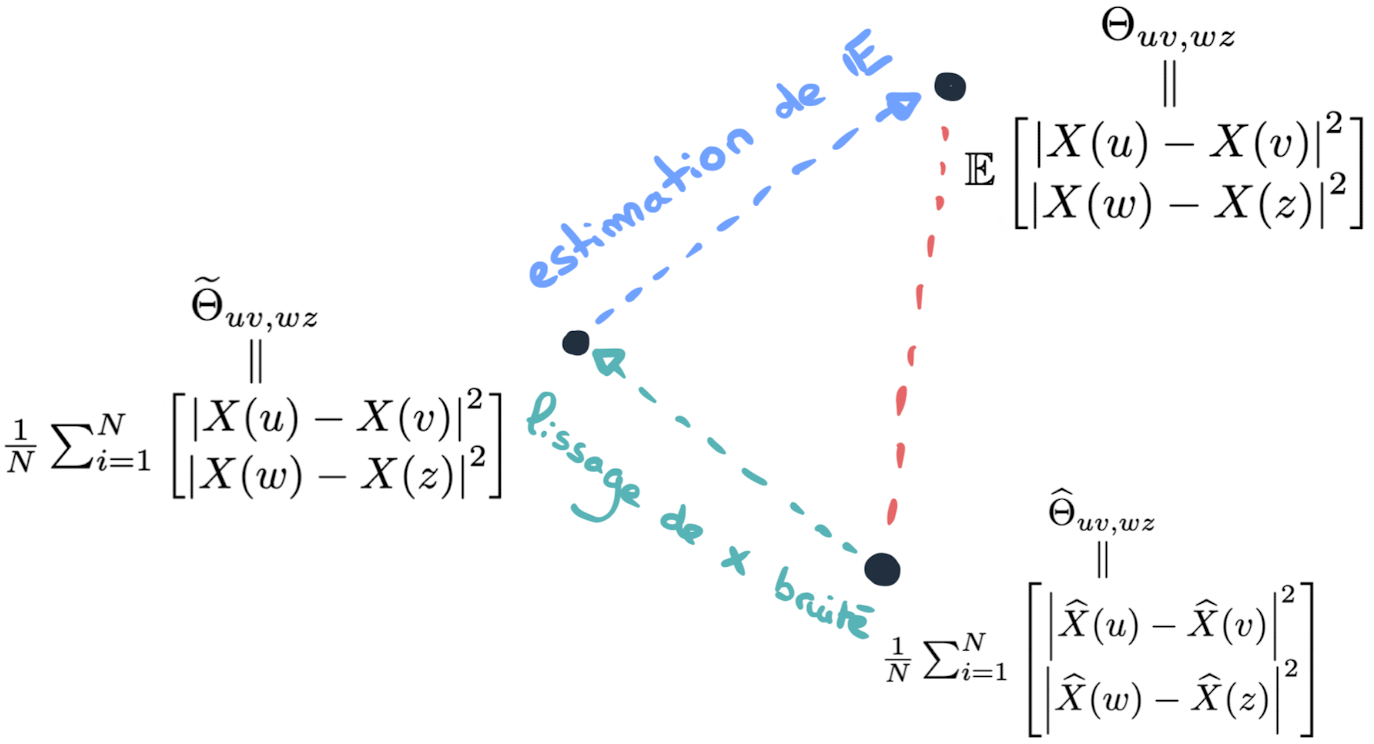
\includegraphics[width=0.7\textwidth]{Images/sketches/theta_biais.png}
	\caption{Schéma représentant les différentes approximations du couple d'incréments}
	\label{fig:sketch_theta_biais}
\end{figure}

\subsection{Choix du Risque}

\subsubsection{Distance Euclidienne}

Afin de quantifier la qualité de l'estimation conjointe du couple de $\theta$, il est raisonnable de considérer la distance euclidienne usuelle pour des vecteurs de $\R 2$

\begin{equation*}
R(\Theta, \Delta) = {\distnorme 2 {\widehat \Theta(\Delta)} {\widetilde \Theta(\Delta)}}^2
\end{equation*}

% et on nomme $R\cindexA(\Delta) = R( \thetaA , \, \Delta \, )$ et $R\cindexB(\Delta) = R( \thetaB, \, \Delta \, )$

\subsubsection{Distance Euclidienne Relative}

On va cependant considérer le risque relatif à la norme de la quantité que l'on cible :

\begin{equation*}
R(\Theta, \Delta) =\frac{ {\distnorme 2 {\widehat \Theta(\Delta)} {\widetilde \Theta(\Delta)}}^2}{ {\norme 2 {\widetilde \Theta(\Delta)}}^2 }
\end{equation*}

\question{Pourquoi considérer la distance euclidienne relative à la norme de la cible $\widetilde \Theta$ plutôt que la distance euclidienne classique qui est plus simple ?}

Le risque sert à déterminer la qualité de l'estimation du couple $\widetilde \Theta$ par $\widehat \Theta$ à un $\Delta$ donné. Il faut cependant garder à l'esprit que $\Theta$ est en réalité une fonction de $\Delta$ car la valeur de $t_1, t_2, t_3$ dépendent de $\Delta$. Ainsi la norme de $\widetilde \Theta$ va varier lorsque l'on fait varier $\Delta$\footnote{il est possible d'obtenir plus de détails en annexe \ref{annexe:tous_theta_conviennent_borne_norme_theta}}. Les risques obtenus via la norme euclidienne sont des risques qui mesurent une différence absolue, mais alors avoir un risque plus petit qu'un autre n'a pas le même sens pour différents $\Delta$ en termes de qualité d'approximation. C'est pourquoi nous considérons le risque relatif dans la détermination du critère du choix du $\Delta$.

On pourra cependant observer la différence entre le risque euclidien et le risque euclidien relatif à la norme de la cible en $\Delta$ sur les figures \ref{fig:sparse_osef} et \ref{fig:sparse_osef_rel}.